\documentclass[letterpaper,10pt,draftclsnofoot,onecolumn,compsoc]{IEEEtran}
\usepackage{graphicx}
\usepackage{amssymb}
\usepackage{amsmath}
\usepackage{array}
\usepackage{amsthm}
\usepackage{listings}
\usepackage{alltt}
\usepackage{float}
\usepackage{color}
\usepackage{url}
\usepackage{setspace}
\usepackage{balance}
\usepackage{enumitem}
\usepackage{pstricks, pst-node}
\usepackage{inputenc}
\usepackage[margin=.75in]{geometry}

\newcommand{\subparagraph}{}
\usepackage{titlesec}

\usepackage{fancyhdr}
\usepackage{hyperref}
\usepackage{tocloft}

\lstset{language=HTML,
        showstringspaces=false}

%hide toc subsubsections
\setcounter{tocdepth}{2}
\setlength{\parindent}{.0in}

%toc formatting for IEEE 830-1998 standards
\renewcommand{\cftsecleader}{\cftdotfill{\cftdotsep}{\vspace{.25cm}}}
\renewcommand{\cftsecfont}{\normalfont}
\renewcommand{\cftsecpagefont}{\normalfont}
\renewcommand{\cftsecaftersnum}{.}

%bottom right page numbers
\fancyhf{}
\renewcommand{\headrulewidth}{0pt}
\rfoot{\thepage}
\pagestyle{fancy}

%formatting specific IEEE 830-1998 Section headings
\titleformat{\section}[block]
  {\fontsize{12}{10}\bfseries\sffamily}
  {\thesection.}
  {1em}
  {}
\titleformat{\subsection}[block]
  {\fontsize{10}{10}\bfseries\sffamily}
  {\thesubsection}
  {1em}
  {\vspace{.1cm}}
\titleformat{\subsubsection}[block]
  {\fontsize{10}{10}\bfseries\sffamily}
  {\thesubsubsection}
  {1em}
  {\vspace{.2cm}}

\newcommand{\cred}[1]{{\color{red}#1}}
\newcommand{\cblue}[1]{{\color{blue}#1}}

\def\name{Charles Siebert, Branden Berlin, Yipeng "Roger" Song}

%% The following metadata will show up in the PDF properties
\hypersetup{
  urlcolor = black,
  pdfauthor = {\name},
  pdfkeywords = {cs461 ``Senior Capstone - Fall 2016'' capstone},
  pdftitle = {CS 461 Requirements Document},
  pdfsubject = {Capstone Requirements Document},
  pdfpagemode = UseNone
}

\begin{document}
\begin{titlepage}
\centering
\vspace*{6cm}
{\scshape\LARGE \begin{singlespace}Optimizing Virtual Reality and Augmented Reality Performance on Mobile Web Applications \\ \end{singlespace} Design Document } \\
	{\scshape\Large CS461 - Fall 2016 \par}
	\vspace{.5cm}
	\name \par
    {\large \today \par} 
	\vspace*{1cm}
	
\begin{abstract}
The technology of Virtual Reality (VR) currently is not cost effective to today's market, as the cost of high-end setups required makes it difficult to afford. Browser developers are focusing primarily on expensive high-end high-performance hardware over mobile devices for Augmented Reality (AR) or Virtual Reality (VR) on the web. Doing AR/VR on the mobile web allows more developers to enter the field and deliver to more customers. To accomplish this, we are working on a project called �Mobile AR/VR Performance�, which focuses on researching to profile and identify performance bottlenecks in 3D web content on mobile devices. We will file issues in the open source projects for Chrome, Firefox through A-Frame and Three.js to determine and identify those bottlenecks. We hope to accomplish this by reporting the challenges and opportunities for performance VR/AR applications, and write a blog post detailing the project results and their best-practices.
\end{abstract}

\end{titlepage}

\newpage

\tableofcontents

%removes page number on table of contents
\thispagestyle{empty}

\newpage

\section{Introduction}
\begin{singlespace}

\par Our project "Optimizing Virtual Reality and Augmented Reality Performance on Mobile Web Applications," nicknamed "OVRAR" is the development of a VR application and analyzing the performance based on the restrictions of using it in a mobile environment with the same devices. Using the data we collect from the application, we can determine specific bottlenecks and performance issues that may be incurred on the device based on different test implementations. This design document is the roadmap of our project for the rest of the year. We will follow the timeline which has been discussed in this document strictly to keep us on the right track. Though little things may change in terms of detail, but the big picture will still be relevant. In this document, we will write up the design of nine pieces that have been discussed from the technology review. The design for each piece will include: describing design components and steps, creating and formatting a glossary; integrating multiple descriptions of design into a full document, referring to past learning (software engineering experience), and identifying appropriate language to fit genre (research project or product development project).

\end{singlespace}

\subsection{Scope}
\begin{singlespace}
\noindent
Optimizing VR and AR for Mobile Web Apps is to determine Virtual Reality (VR) and Augmented Reality (AR) bottlenecks that exist in mobile devices within the A-Frame framework. The bottlenecks can be caused from either unoptimized development of software, underpowered or unoptimized hardware found in existing devices, or potential bugs or limitations found within the framework itself. The software itself, which is developed on A-Frame, will generate multiple scenes where it will test the graphical capabilities of the hardware within the mobile devices, the types of different implementations of certain scenes, and determine areas of optimization through these multiple scenes. The software will be used to create a report that will analyze the information collected about processing power, frame rates, battery usage, and the limitations of the framework to determine the best practices for implementing more graphically intensive programs on A-Frame. \\

\noindent
Developers other than us will use the information in the report to determine the best way to approach at designing their programs, as the software we create will only serve as test cases and stress testing for mobile devices to collect this information. 
\end{singlespace}

\subsection{Purpose}
\begin{singlespace}
\noindent
The purpose of this project is to determine areas of development within A-Frame where practices will be best used, as they will least be likely to impede on bottle necking either the software or hardware whe n optimizing the software for performance. This project is focused towards the advancement of an open-source, developing web framework, and the developers making their own products with A-Frame and for mobile devices. The developers will be using our project research as a means to avoid these bottlenecks in this evolving environment.
\end{singlespace}

\subsection{Glossary}
\begin{singlespace}
\begin{enumerate}[labelsep=2em,leftmargin=.5in]
    {\item \bfseries Virtual Reality (VR): } Computer generated three-dimensional environment that immerses the user into the environment using special equipment or implementation techniques. \vspace{.1cm}
    {\item \bfseries Augmented Reality (AR): } Provides a composite view to the user based on computer generated environments super-imposed onto the view of the real world. \vspace{.1cm}
    {\item \bfseries Operating System (OS): } Software that supports an interface to support computer's basic functions, such as process scheduling, executing tasks, and allowing user interface. Specifically this project is in regards to Android OS. \vspace{.1cm}
    {\item \bfseries Web Framework: } A software framework that is designed to support the development of web applications including web services, web resources and web APIs. \vspace{.1cm}
    {\item \bfseries A-Frame: } A-Frame is an open-source WebVR framework for creating virtual reality (VR) experiences with HTML with the use of the Three.js framework.\vspace{.1cm}
    {\item \bfseries Three.js: } JavaScript framework that allows accessible development WebGL applications. \vspace{.1cm}
    {\item \bfseries WebGL: } JavaScript API that allows for rendering interactive 3D and 2D computer graphics within any compatible web browser without the use of plug-ins. \vspace{.1cm}
    {\item \bfseries Viewport: } A viewport is a viewing region in computer graphics. This region is defined in the software to allow for viewing the drawing of objects. This viewport is typically bounded by a window or by the full screen of the mobile device. \vspace{.1cm}
    {\item \bfseries Local Web Server: } A webs erver for hosting web page content to allow access on local networks, without having to go out into the internet to access the information. \vspace{.1cm}
    {\item \bfseries Hosted Web Server: } A server that is hosted externally on the internet, where it holds and displays the web information, needing to go out to the internet, and back again to receive the proper information. \vspace{.1cm}
    {\item \bfseries Implementation Languages: } a formal computer language or constructed language designed to communicate instructions to a machine, particularly a computer. i.e. HTML, JavaScript, C, C++, etc. \vspace{.1cm}
    {\item \bfseries Mobile Devices: } A device that is able to be held and portable by a user, typically a smart phone or table.t\vspace{.1cm}
    {\item \bfseries Rendering: } Part of the graphical process that draws everything into the "view's" scene. This includes textures, animations, objects, surface information, etc. \vspace{.1cm}
    {\item \bfseries Bottleneck: } An effect impeding on the rendering process, which occurs between the hardware and software aspects. \vspace{.1cm}
    {\item \bfseries Optimize: } Process of making something as fully functional or effective as possible, including the types of limitations that occur in the environment. \vspace{.1cm}
    {\item \bfseries Performance: } The process of how well the software handles the action or function of the software.
    {\item \bfseries Software Bug: } An error, flaw, failure or fault in the system that causes it to produce an incorrect or unexpected result, or to behave in unintended ways. \vspace{.1cm}
    %{\item \bfseries [word]: } Something \vspace{.1cm}
\end{enumerate}

\end{singlespace}
\section{Utilization Of Technologies}
\begin{singlespace}
\subsection{Browser Scene Generation via Mozilla Firefox}
\par The web browser we will be using is Mozilla Firefox. Firefox is currently the best supported browser for our A-Frame open source library and WebGL API. The VR experience in this browser is a temporary mode within the original and familiar 2D interface. Because it is a temporary mode and not a full immersion, we will be able to navigate a familiar GUI allowing us to comfortably and seamlessly investigate builds and returned data. Additionally, the Developer Edition of Firefox will give us built in tools for debugging the mobile web browser experience in hopes to have a more guided and straightforward data return. Additionally, the code necessary to begin our research can be minimal due to Firefox�s VR ready libraries. Firefox, combined with A-Frame, will allow us to create a VR site by simply placing a single line of HTML in our locally run server.
\begin{figure}[H]
\caption{Sample HTML}
\begin{lstlisting}
<!DOCTYPE html>
<html>
    <head>
        <meta charset="utf-8">
        <title>My first VR site</title>
        <script src="https://aframe.io/releases/latest/aframe.min.js"></script>
    </head>
    <body>
        <a-scene>
        </a-scene>
    </body>
</html>
\end{lstlisting} 
\end{figure}
\par Additionally, objects can be added to this mock up via simple scene inputs
\begin{figure}[H]
\caption{Sample Scene Generation HTML}
\begin{lstlisting}
<a-scene>
    <a-sphere position="0 1.25 -1" radius="1.25" color="#EF2D5E"></a-sphere>
    <a-cube position="-1 0.5 1" rotation="0 45 0" width="1" height="1" depth="1"
        color="#4CC3D9"></a-cube>
    <a-cylinder position="1 0.75 1" radius="0.5" height="1.5" color="#FFC65D"></a-cylinder>
    <a-plane rotation="-90 0 0" width="4" height="4" color="#7BC8A4"></a-plane>
    <a-sky color="#ECECEC"></a-sky>
</a-scene>
\end{lstlisting} 
\end{figure}
\par This allows us to place lines on the fly and have their presentations appear real-time. Because of the Firefox/A-Frame combination, we do not have to worry about old �agreed upon standards� or worry about lack of support from the actual experience. The integration is flawless and fluidity of our testing will allow us to explore uncharted territory and get creative with our research.

\subsection{Lochost Server Setup via Apache}
\par We will be using Apache HTTP to host our local web server for testing because of its ability to deliver web pages upon immediate request to its clients. We will be injecting, deleting, altering code quickly and need a server application that will give us immediate results. Additionally, Apache allows the creating of virtualhosts. With VH, we will be able to designate a virtual host on our server giving the appearance of many different different hosts on a single IP address. This means that we can potentially work concurrently without the need of all of use physically being present. The Apache VH allows us to designate other servers and route them to our main server for combined testing and web hosting. Additionally, and most importantly, Apache supports load balancing. Load balancing is the ability to balance traffic coming in a cluster, dividing traffic evenly among all members utilizing the server. Some more benefits of using Apache as our sole localhost are that it has a long history of reliability and performance, meaning that there is copious amounts of documentation so we can get help with things we potential need to troubleshoot. And the best part is it is open source and free!

\subsection{Analyzation and Collection of Data via Microsoft Excel}
\par To analyze our data we are going with the Microsoft Excel. We decided to go this route due Excel�s ability to track leads and analyze data. The lead-track holds data collection capabilities through worksheets and a series of �PivotTables� that analyze the input of data and offer a summarization details. The best part is that the learning curve for the capabilities is relatively small. The data storage is straightforward and the manipulation of said data via formulas allows us to apply perform calculations, track averages, and format related cells all on the fly. Another benefit of Excel is the local storage of data. Additionally, along wiht the storage of data, Excel allows us to explore possible outcomes by using its what-of tools to manipulate data within the sheet itself, combining it with some of its many complex calculation formulas to run what-if scenarios on our numbers to hopefully give us expected outcomes before we even implement them as well as giving us data for several scenarios. Finally, as a spreadsheet program, Excel can store millions of tables of data (not that we will have that much) allowing us to run comparisons of data, create improvement charts for visual representations, and run statistic, engineering, and regression analysis. 

\end{singlespace}
\section{Program Implementation}
\begin{singlespace}
\par Our beginning implementation of this research project is going to depend on previous implementations and errors already reported by the Mozilla VR and AR team. We are going to begin by looking at the current issues that have been reported and find the ones that have already been solved, the ones that need investigation, and additionally the areas that not have been looked into in depth. We will do this by utilizing A-Frame to investigate the original three.js framework. We will do this in attempt to recreate the errors that have been reported but not yet fixed, to get a basis of how we will be interacting with this project and what our future error searching will look like. Once we recreate the errors, we will begin to expand. We will build further on the Javascript code by stress testing and narrowing down on the issues through WebGL API interactions, all so we can not only get an idea of what these errors might look like, but also so we don't spend time on on current issues that have already been reported. Then, after getting our bearings with the already reported issues, we will begin to delve into unknown territory. We will not only push further into the reported territory, we will take a step back and shift our focus on to uncharted territory. Once there, we will push the limits of our software, max out their capabilities, and stress every nook and cranny of our software to uncover unexplored issues. These issues will be reported to us via output data related to hardware, software, and general browser generated scenes.
\end{singlespace}

\section{Reiteration Implementation}
\begin{singlespace}
\par For the second half of our implementation, we will continue to delve into the unknown but on top of that we hone in on the specifics of our originally found errors. We will hopefully narrow down on the issues so we can report the exact location, cause, and if we can, the solution. By the end of this project, we hope to have found many issues that plague the web VR and AR experience and we hope to have honed in on the exact cause of them in hopes to provide swift and easy solutions for future dev teams.   
\end{singlespace}

\section{Gantt Chart Information}

\begin{singlespace}

\begin{description}[leftmargin=0in]
\item[Problem Statement:] Detailing the description and proposed solution to the problem for this project.\vspace{.1cm}
\item[Requirements Document:] Detailing the project outline, and the process included within the project.\vspace{.1cm}
\item[Technology Review:] Process within our group to analyze the project's scope, delegate tasks within it, and what we will be handling.\vspace{.1cm}
\item[Design Document:] Document writing detailing how we will be working on this project, including our tools and testing information. \vspace{.1cm}
\item[Initial Implementations:] Our group will be working on setting up our devices, and getting comfortable with mobile development workflow with "Hello World!" \vspace{.1cm}
\item[Progress Report \#1:] A report detailing the progress we've made during our first term within this project.\vspace{.1cm}
\item[Research Bugs and Tools:] Time during winter break, will be spent understanding the optimization issues found in mobile devices with the frameworks, and the bugs that exist. Time is also spent preliminarily working with and understanding the performance measurement tools used for this project.\vspace{.1cm}
\item[Program Design:] After researching and testing initial implementations, this time will be used discussing and designing our specific program implementation, working with the tools to measure performance metrics, and defining the work flow of our program and the tools to receive meaningful results.\vspace{.1cm}
\item[Program Implementation (First Two Week Sprint):] Working in two week sprints, we will be able to focus on implementing features and evaluating the process. This is our first sprint.\vspace{.1cm}
\item[Evaluation and Debug:] First rounds of evaluation, where time is spent analyzing the performance metrics we acquired, plotting what they mean, note and report any blatant optimization issues or bugs.\vspace{.1cm}
\item[Reiterate Implementation (Second Two Week Sprint):] Second two week sprint, where the focus is on improving the performance metrics from our first implementation, and fixing any issues we encountered.\vspace{.1cm}
\item[Evaluation and Debug:] Second rounds of evaluation, where time is spent analyzing the performance metrics we acquired from the second sprints, and comparing the differences between the last rounds of evaluation. \vspace{.1cm}
\item[Progress Report \#2:] A report detailing the progress we've made during our second term within this project.\vspace{.1cm}
\item[Preparing for EXPO:] Long space open to account for future term requirements and uncertainty. This may include an additional sprint and evaluation depending on other unforeseen requirements that need to be met. \vspace{.1cm}
\item[Final Report:] A report detailing the progress we've made during our last term within this project.\vspace{.1cm}
\end{description}

\end{singlespace}

\subsection{Gantt Chart}
\begin{figure}[H]
    \begin{center}
        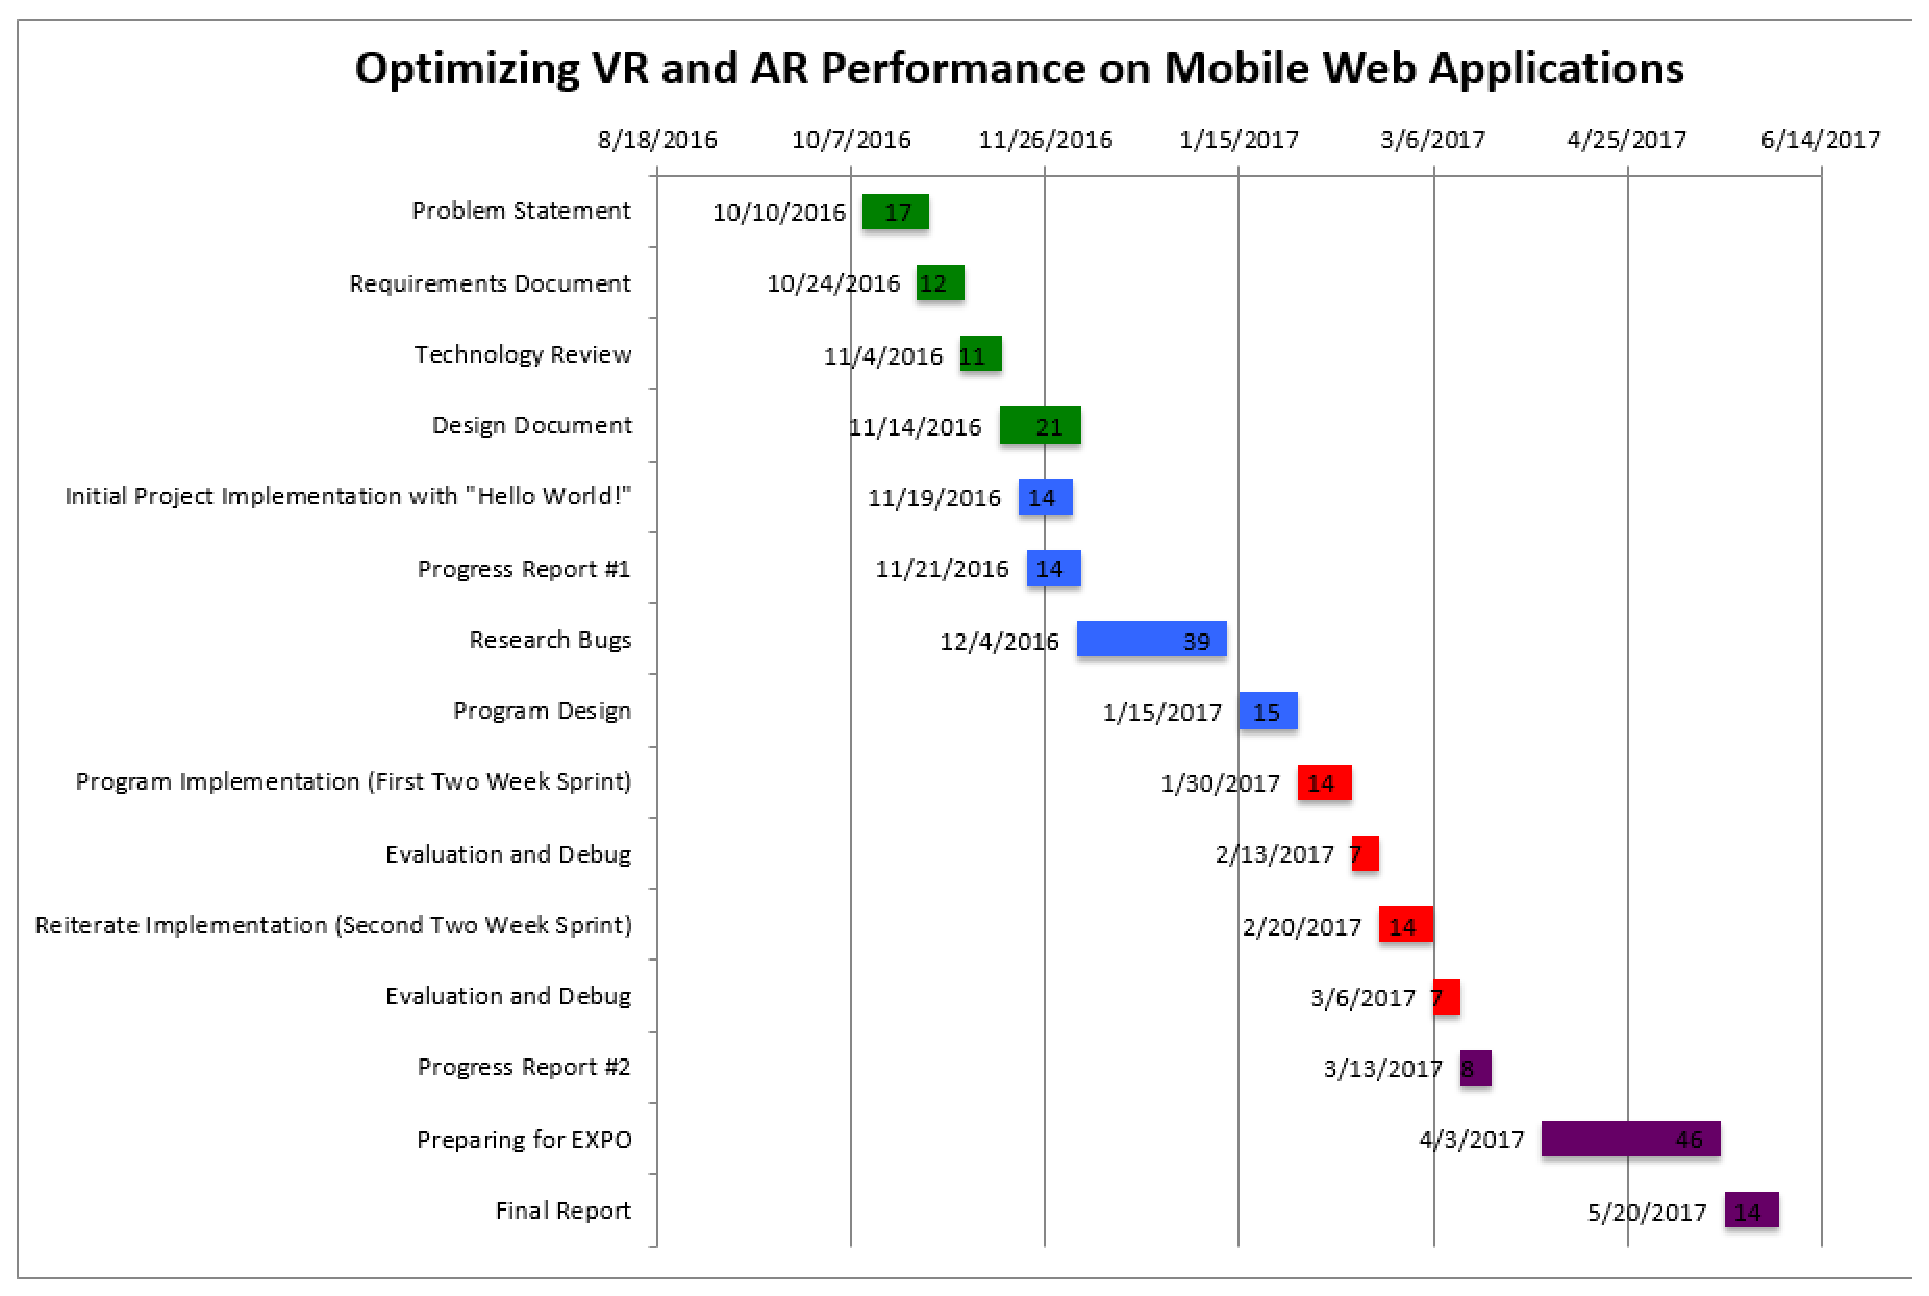
\includegraphics[width=1\textwidth]{OVRAR_Gantt_Chart.eps}
    \end{center}
\end{figure} 
\vfill

\noindent\begin{tabular}{ll}
\makebox[3.5in]{\hrulefill} & \makebox[1.5in]{\hrulefill}\\
Client Signature & Date\\
[4ex]% adds space between the two sets of signatures
\makebox[3.5in]{\hrulefill} & \makebox[1.5in]{\hrulefill}\\
Group Signature & Date\\
[4ex]% adds space between the two sets of signatures
\makebox[3.5in]{\hrulefill} & \makebox[1.5in]{\hrulefill}\\
Group Signature & Date\\
[4ex]% adds space between the two sets of signatures
\makebox[3.5in]{\hrulefill} & \makebox[1.5in]{\hrulefill}\\
Group Signature & Date\\
\end{tabular}
\end{document}